\documentclass[]{article}
\usepackage{lmodern}
\usepackage{amssymb,amsmath}
\usepackage{ifxetex,ifluatex}
\usepackage{fixltx2e} % provides \textsubscript
\ifnum 0\ifxetex 1\fi\ifluatex 1\fi=0 % if pdftex
  \usepackage[T1]{fontenc}
  \usepackage[utf8]{inputenc}
\else % if luatex or xelatex
  \ifxetex
    \usepackage{mathspec}
  \else
    \usepackage{fontspec}
  \fi
  \defaultfontfeatures{Ligatures=TeX,Scale=MatchLowercase}
\fi
% use upquote if available, for straight quotes in verbatim environments
\IfFileExists{upquote.sty}{\usepackage{upquote}}{}
% use microtype if available
\IfFileExists{microtype.sty}{%
\usepackage{microtype}
\UseMicrotypeSet[protrusion]{basicmath} % disable protrusion for tt fonts
}{}
\usepackage[margin=1in]{geometry}
\usepackage{hyperref}
\hypersetup{unicode=true,
            pdftitle={ANOVA desenvolvimento \textasciitilde{} unidade},
            pdfauthor={Geiser C. Challco geiser@usp.br},
            pdfborder={0 0 0},
            breaklinks=true}
\urlstyle{same}  % don't use monospace font for urls
\usepackage{color}
\usepackage{fancyvrb}
\newcommand{\VerbBar}{|}
\newcommand{\VERB}{\Verb[commandchars=\\\{\}]}
\DefineVerbatimEnvironment{Highlighting}{Verbatim}{commandchars=\\\{\}}
% Add ',fontsize=\small' for more characters per line
\usepackage{framed}
\definecolor{shadecolor}{RGB}{248,248,248}
\newenvironment{Shaded}{\begin{snugshade}}{\end{snugshade}}
\newcommand{\AlertTok}[1]{\textcolor[rgb]{0.94,0.16,0.16}{#1}}
\newcommand{\AnnotationTok}[1]{\textcolor[rgb]{0.56,0.35,0.01}{\textbf{\textit{#1}}}}
\newcommand{\AttributeTok}[1]{\textcolor[rgb]{0.77,0.63,0.00}{#1}}
\newcommand{\BaseNTok}[1]{\textcolor[rgb]{0.00,0.00,0.81}{#1}}
\newcommand{\BuiltInTok}[1]{#1}
\newcommand{\CharTok}[1]{\textcolor[rgb]{0.31,0.60,0.02}{#1}}
\newcommand{\CommentTok}[1]{\textcolor[rgb]{0.56,0.35,0.01}{\textit{#1}}}
\newcommand{\CommentVarTok}[1]{\textcolor[rgb]{0.56,0.35,0.01}{\textbf{\textit{#1}}}}
\newcommand{\ConstantTok}[1]{\textcolor[rgb]{0.00,0.00,0.00}{#1}}
\newcommand{\ControlFlowTok}[1]{\textcolor[rgb]{0.13,0.29,0.53}{\textbf{#1}}}
\newcommand{\DataTypeTok}[1]{\textcolor[rgb]{0.13,0.29,0.53}{#1}}
\newcommand{\DecValTok}[1]{\textcolor[rgb]{0.00,0.00,0.81}{#1}}
\newcommand{\DocumentationTok}[1]{\textcolor[rgb]{0.56,0.35,0.01}{\textbf{\textit{#1}}}}
\newcommand{\ErrorTok}[1]{\textcolor[rgb]{0.64,0.00,0.00}{\textbf{#1}}}
\newcommand{\ExtensionTok}[1]{#1}
\newcommand{\FloatTok}[1]{\textcolor[rgb]{0.00,0.00,0.81}{#1}}
\newcommand{\FunctionTok}[1]{\textcolor[rgb]{0.00,0.00,0.00}{#1}}
\newcommand{\ImportTok}[1]{#1}
\newcommand{\InformationTok}[1]{\textcolor[rgb]{0.56,0.35,0.01}{\textbf{\textit{#1}}}}
\newcommand{\KeywordTok}[1]{\textcolor[rgb]{0.13,0.29,0.53}{\textbf{#1}}}
\newcommand{\NormalTok}[1]{#1}
\newcommand{\OperatorTok}[1]{\textcolor[rgb]{0.81,0.36,0.00}{\textbf{#1}}}
\newcommand{\OtherTok}[1]{\textcolor[rgb]{0.56,0.35,0.01}{#1}}
\newcommand{\PreprocessorTok}[1]{\textcolor[rgb]{0.56,0.35,0.01}{\textit{#1}}}
\newcommand{\RegionMarkerTok}[1]{#1}
\newcommand{\SpecialCharTok}[1]{\textcolor[rgb]{0.00,0.00,0.00}{#1}}
\newcommand{\SpecialStringTok}[1]{\textcolor[rgb]{0.31,0.60,0.02}{#1}}
\newcommand{\StringTok}[1]{\textcolor[rgb]{0.31,0.60,0.02}{#1}}
\newcommand{\VariableTok}[1]{\textcolor[rgb]{0.00,0.00,0.00}{#1}}
\newcommand{\VerbatimStringTok}[1]{\textcolor[rgb]{0.31,0.60,0.02}{#1}}
\newcommand{\WarningTok}[1]{\textcolor[rgb]{0.56,0.35,0.01}{\textbf{\textit{#1}}}}
\usepackage{longtable,booktabs}
\usepackage{graphicx,grffile}
\makeatletter
\def\maxwidth{\ifdim\Gin@nat@width>\linewidth\linewidth\else\Gin@nat@width\fi}
\def\maxheight{\ifdim\Gin@nat@height>\textheight\textheight\else\Gin@nat@height\fi}
\makeatother
% Scale images if necessary, so that they will not overflow the page
% margins by default, and it is still possible to overwrite the defaults
% using explicit options in \includegraphics[width, height, ...]{}
\setkeys{Gin}{width=\maxwidth,height=\maxheight,keepaspectratio}
\IfFileExists{parskip.sty}{%
\usepackage{parskip}
}{% else
\setlength{\parindent}{0pt}
\setlength{\parskip}{6pt plus 2pt minus 1pt}
}
\setlength{\emergencystretch}{3em}  % prevent overfull lines
\providecommand{\tightlist}{%
  \setlength{\itemsep}{0pt}\setlength{\parskip}{0pt}}
\setcounter{secnumdepth}{0}
% Redefines (sub)paragraphs to behave more like sections
\ifx\paragraph\undefined\else
\let\oldparagraph\paragraph
\renewcommand{\paragraph}[1]{\oldparagraph{#1}\mbox{}}
\fi
\ifx\subparagraph\undefined\else
\let\oldsubparagraph\subparagraph
\renewcommand{\subparagraph}[1]{\oldsubparagraph{#1}\mbox{}}
\fi

%%% Use protect on footnotes to avoid problems with footnotes in titles
\let\rmarkdownfootnote\footnote%
\def\footnote{\protect\rmarkdownfootnote}

%%% Change title format to be more compact
\usepackage{titling}

% Create subtitle command for use in maketitle
\providecommand{\subtitle}[1]{
  \posttitle{
    \begin{center}\large#1\end{center}
    }
}

\setlength{\droptitle}{-2em}

  \title{ANOVA \texttt{desenvolvimento} \textasciitilde{} \texttt{unidade}}
    \pretitle{\vspace{\droptitle}\centering\huge}
  \posttitle{\par}
    \author{Geiser C. Challco \href{mailto:geiser@usp.br}{\nolinkurl{geiser@usp.br}}}
    \preauthor{\centering\large\emph}
  \postauthor{\par}
    \date{}
    \predate{}\postdate{}
  

\begin{document}
\maketitle

\begin{itemize}
\tightlist
\item
  Report as Word format: \url{factorialAnova.docx}
\item
  Report as LaTex format: \url{factorialAnova.tex}
\end{itemize}

\hypertarget{initial-data-and-preprocessing}{%
\subsection{Initial Data and
Preprocessing}\label{initial-data-and-preprocessing}}

R script: \url{factorialAnova.R} Inital data: \url{data.csv}

\hypertarget{summary-statistics-of-the-initial-data}{%
\subsubsection{Summary statistics of the initial
data}\label{summary-statistics-of-the-initial-data}}

\begin{Shaded}
\begin{Highlighting}[]
\KeywordTok{get_summary_stats}\NormalTok{(}\KeywordTok{group_by}\NormalTok{(dat, }\StringTok{`}\DataTypeTok{unidade}\StringTok{`}\NormalTok{), }\DataTypeTok{type =}\StringTok{"common"}\NormalTok{)}
\end{Highlighting}
\end{Shaded}

\begin{verbatim}
## # A tibble: 3 x 11
##   unidade   variable     n   min   max median   iqr  mean    sd    se    ci
##   <fct>     <chr>    <dbl> <dbl> <dbl>  <dbl> <dbl> <dbl> <dbl> <dbl> <dbl>
## 1 UFAL A.C~ desenvo~   241     1  4.33   2.67  1.33  2.69 0.827 0.053 0.105
## 2 UFAL Ara~ desenvo~    55     1  5      2.67  1.17  2.62 0.871 0.117 0.236
## 3 UFAL CECA desenvo~    24     1  4.67   2.67  1.08  2.71 0.939 0.192 0.397
\end{verbatim}

\hypertarget{check-assumptions}{%
\subsection{Check Assumptions}\label{check-assumptions}}

\hypertarget{identifying-outliers}{%
\subsubsection{Identifying outliers}\label{identifying-outliers}}

Outliers tend to increase type-I error probability, and they decrease
the calculated F statistic in ANOVA resulting in a lower chance of
reject the null hypothesis.

\begin{itemize}
\tightlist
\item
  Identified outliers using rstatix
\end{itemize}

\begin{Shaded}
\begin{Highlighting}[]
\KeywordTok{identify_outliers}\NormalTok{(}\KeywordTok{group_by}\NormalTok{(dat, }\StringTok{`}\DataTypeTok{unidade}\StringTok{`}\NormalTok{), }\StringTok{`}\DataTypeTok{desenvolvimento}\StringTok{`}\NormalTok{)}
\end{Highlighting}
\end{Shaded}

\begin{verbatim}
## # A tibble: 1 x 5
##   unidade        ID     desenvolvimento is.outlier is.extreme
##   <fct>          <fct>            <dbl> <lgl>      <lgl>     
## 1 UFAL Arapiraca Obs322               5 TRUE       FALSE
\end{verbatim}

\begin{itemize}
\tightlist
\item
  Identified outliers through Boxplots
\end{itemize}

\begin{Shaded}
\begin{Highlighting}[]
\KeywordTok{Boxplot}\NormalTok{(}\StringTok{`}\DataTypeTok{desenvolvimento}\StringTok{`} \OperatorTok{~}\StringTok{ `}\DataTypeTok{unidade}\StringTok{`}\NormalTok{, }\DataTypeTok{data =}\NormalTok{ dat, }\DataTypeTok{id =} \KeywordTok{list}\NormalTok{(}\DataTypeTok{n =} \OtherTok{Inf}\NormalTok{))}
\end{Highlighting}
\end{Shaded}

\includegraphics{factorialAnova_files/figure-latex/unnamed-chunk-3-1.pdf}

\begin{verbatim}
## [1] "Obs322"
\end{verbatim}

\hypertarget{removing-outliers-from-the-data}{%
\subsubsection{Removing outliers from the
data}\label{removing-outliers-from-the-data}}

\begin{Shaded}
\begin{Highlighting}[]
\NormalTok{outliers <-}\StringTok{ }\KeywordTok{c}\NormalTok{(}\StringTok{"Obs322"}\NormalTok{)}
\NormalTok{rdat <-}\StringTok{ }\NormalTok{dat[}\OperatorTok{!}\NormalTok{dat[[}\StringTok{"ID"}\NormalTok{]] }\OperatorTok\StringTok{ }\NormalTok{outliers,]   }\CommentTok{# table without outliers}
\end{Highlighting}
\end{Shaded}

\begin{longtable}[]{@{}lllr@{}}
\caption{Outliers table}\tabularnewline
\toprule
& ID & unidade & desenvolvimento\tabularnewline
\midrule
\endfirsthead
\toprule
& ID & unidade & desenvolvimento\tabularnewline
\midrule
\endhead
Obs322 & Obs322 & UFAL Arapiraca & 5\tabularnewline
\bottomrule
\end{longtable}

\hypertarget{normality-assumption}{%
\subsubsection{Normality assumption}\label{normality-assumption}}

\textbf{Observation}:

As sample sizes increase, ANOVA remains a valid test even with the
violation of normality {[}\protect\hyperlink{references}{1},
\protect\hyperlink{references}{2}{]}. According to the central limit
theorem, the sampling distribution tends to be normal if the sample is
large enough (\texttt{n\ \textgreater{}\ 30}). Therefore, we performed
ANOVA with large samples as follows:

\begin{itemize}
\item
  In cases with the sample size greater than 30
  (\texttt{n\ \textgreater{}\ 30}), we adopted a significance level of
  \texttt{p\ \textless{}\ 0.01} instead a significance level of
  \texttt{p\ \textless{}\ 0.05}.
\item
  For samples with \texttt{n\ \textgreater{}\ 50} observation, we
  adopted D'Agostino-Pearson test that offers better accuracy for larger
  samples {[}\protect\hyperlink{references}{3}{]}.
\item
  For samples' size between \texttt{n\ \textgreater{}\ 100} and
  \texttt{n\ \textless{}=\ 200}, we ignored both tests (Shapiro and
  D'Agostino-Persons), and our decision of normality were based only in
  the interpretation of QQ-plots and histograms because these tests tend
  to be too sensitive with values greater than 200
  {[}\protect\hyperlink{references}{3}{]}.
\item
  For samples with \texttt{n\ \textgreater{}\ 200} observation, we
  ignore the normality assumption based on the central theorem limit,
  and taking only into account the homogeneity assumption.
\end{itemize}

\hypertarget{checking-normality-assumption-in-the-residual-model}{%
\paragraph{Checking normality assumption in the residual
model}\label{checking-normality-assumption-in-the-residual-model}}

\begin{Shaded}
\begin{Highlighting}[]
\NormalTok{mdl <-}\StringTok{ }\KeywordTok{lm}\NormalTok{(}\StringTok{`}\DataTypeTok{desenvolvimento}\StringTok{`} \OperatorTok{~}\StringTok{ `}\DataTypeTok{unidade}\StringTok{`}\NormalTok{, }\DataTypeTok{data =}\NormalTok{ rdat)}
\KeywordTok{normality_test}\NormalTok{(}\KeywordTok{residuals}\NormalTok{(mdl))}
\end{Highlighting}
\end{Shaded}

\begin{verbatim}
##     n statistic     method            p p.signif normality
## 1 319  13.90795 D'Agostino 0.0009548309       **         -
\end{verbatim}

The QQ plot used to evaluate normality assumption

\begin{Shaded}
\begin{Highlighting}[]
\KeywordTok{qqPlot}\NormalTok{(}\KeywordTok{residuals}\NormalTok{(mdl))}
\end{Highlighting}
\end{Shaded}

\includegraphics{factorialAnova_files/figure-latex/unnamed-chunk-7-1.pdf}

\begin{verbatim}
## Obs278 Obs254 
##    271    248
\end{verbatim}

\hypertarget{checking-normality-assumption-for-each-group}{%
\paragraph{Checking normality assumption for each
group}\label{checking-normality-assumption-for-each-group}}

\begin{Shaded}
\begin{Highlighting}[]
\KeywordTok{normality_test_at}\NormalTok{(}\KeywordTok{group_by}\NormalTok{(rdat, }\StringTok{`}\DataTypeTok{unidade}\StringTok{`}\NormalTok{), }\StringTok{"desenvolvimento"}\NormalTok{)}
\end{Highlighting}
\end{Shaded}

\begin{verbatim}
##                      variable          unidade   n  statistic       method
## 1             desenvolvimento UFAL A.C. Simões 241 12.1413615   D'Agostino
## Omnibus  Test desenvolvimento   UFAL Arapiraca  54  2.1184303   D'Agostino
## 11            desenvolvimento        UFAL CECA  24  0.9780299 Shapiro-Wilk
##                       p p.signif normality
## 1             0.0023096        *         -
## Omnibus  Test 0.3467278       ns       YES
## 11            0.8569623       ns       YES
\end{verbatim}

\begin{itemize}
\tightlist
\item
  QQ plot in the \textbf{unidade}: ``UFAL A.C. Simões''
\end{itemize}

\begin{Shaded}
\begin{Highlighting}[]
\KeywordTok{qqPlot}\NormalTok{( }\OperatorTok{~}\StringTok{ `}\DataTypeTok{desenvolvimento}\StringTok{`}\NormalTok{, }\DataTypeTok{data =}\NormalTok{ rdat[}\KeywordTok{which}\NormalTok{(rdat[}\StringTok{"unidade"}\NormalTok{] }\OperatorTok{==}\StringTok{ "UFAL A.C. Simões"),])}
\end{Highlighting}
\end{Shaded}

\includegraphics{factorialAnova_files/figure-latex/unnamed-chunk-9-1.pdf}

\begin{verbatim}
## Obs10 Obs49 
##     8    41
\end{verbatim}

\begin{itemize}
\tightlist
\item
  QQ plot in the \textbf{unidade}: ``UFAL Arapiraca''
\end{itemize}

\begin{Shaded}
\begin{Highlighting}[]
\KeywordTok{qqPlot}\NormalTok{( }\OperatorTok{~}\StringTok{ `}\DataTypeTok{desenvolvimento}\StringTok{`}\NormalTok{, }\DataTypeTok{data =}\NormalTok{ rdat[}\KeywordTok{which}\NormalTok{(rdat[}\StringTok{"unidade"}\NormalTok{] }\OperatorTok{==}\StringTok{ "UFAL Arapiraca"}\NormalTok{),])}
\end{Highlighting}
\end{Shaded}

\includegraphics{factorialAnova_files/figure-latex/unnamed-chunk-10-1.pdf}

\begin{verbatim}
## Obs254 Obs269 
##     42     44
\end{verbatim}

\begin{itemize}
\tightlist
\item
  QQ plot in the \textbf{unidade}: ``UFAL CECA''
\end{itemize}

\begin{Shaded}
\begin{Highlighting}[]
\KeywordTok{qqPlot}\NormalTok{( }\OperatorTok{~}\StringTok{ `}\DataTypeTok{desenvolvimento}\StringTok{`}\NormalTok{, }\DataTypeTok{data =}\NormalTok{ rdat[}\KeywordTok{which}\NormalTok{(rdat[}\StringTok{"unidade"}\NormalTok{] }\OperatorTok{==}\StringTok{ "UFAL CECA"}\NormalTok{),])}
\end{Highlighting}
\end{Shaded}

\includegraphics{factorialAnova_files/figure-latex/unnamed-chunk-11-1.pdf}

\begin{verbatim}
## Obs278 Obs239 
##     18     16
\end{verbatim}

\hypertarget{removing-data-that-affect-normality}{%
\paragraph{Removing data that affect
normality}\label{removing-data-that-affect-normality}}

\begin{Shaded}
\begin{Highlighting}[]
\NormalTok{non.normal <-}\StringTok{ }\KeywordTok{c}\NormalTok{(}\StringTok{""}\NormalTok{)}
\NormalTok{sdat <-}\StringTok{ }\NormalTok{rdat[}\OperatorTok{!}\NormalTok{rdat[[}\StringTok{"ID"}\NormalTok{]] }\OperatorTok\StringTok{ }\NormalTok{non.normal,]   }\CommentTok{# table without non-normal and outliers}
\end{Highlighting}
\end{Shaded}

\begin{longtable}[]{@{}llr@{}}
\caption{Non-normal data table}\tabularnewline
\toprule
ID & unidade & desenvolvimento\tabularnewline
\midrule
\endfirsthead
\toprule
ID & unidade & desenvolvimento\tabularnewline
\midrule
\endhead
\bottomrule
\end{longtable}

\hypertarget{performing-normality-test-without-data-that-affect-normality}{%
\paragraph{Performing normality test without data that affect
normality}\label{performing-normality-test-without-data-that-affect-normality}}

\begin{Shaded}
\begin{Highlighting}[]
\NormalTok{mdl <-}\StringTok{ }\KeywordTok{lm}\NormalTok{(}\StringTok{`}\DataTypeTok{desenvolvimento}\StringTok{`} \OperatorTok{~}\StringTok{ `}\DataTypeTok{unidade}\StringTok{`}\NormalTok{, }\DataTypeTok{data =}\NormalTok{ sdat)}
\KeywordTok{normality_test}\NormalTok{(}\KeywordTok{residuals}\NormalTok{(mdl))}
\end{Highlighting}
\end{Shaded}

\begin{longtable}[]{@{}rrllll@{}}
\toprule
n & statistic & method & p & p.signif & normality\tabularnewline
\midrule
\endhead
319 & 13.908 & D'Agostino & 0.001 & ** & -\tabularnewline
\bottomrule
\end{longtable}

\begin{Shaded}
\begin{Highlighting}[]
\KeywordTok{normality_test_at}\NormalTok{(}\KeywordTok{group_by}\NormalTok{(sdat, }\StringTok{`}\DataTypeTok{unidade}\StringTok{`}\NormalTok{), }\StringTok{"desenvolvimento"}\NormalTok{)}
\end{Highlighting}
\end{Shaded}

\begin{longtable}[]{@{}llrrllll@{}}
\toprule
variable & unidade & n & statistic & method & p & p.signif &
normality\tabularnewline
\midrule
\endhead
desenvolvimento & UFAL A.C. Simões & 241 & 12.1414 & D'Agostino & 0.0023
& ** & -\tabularnewline
desenvolvimento & UFAL Arapiraca & 54 & 2.1184 & D'Agostino & 0.3467 &
ns & YES\tabularnewline
desenvolvimento & UFAL CECA & 24 & 0.9780 & Shapiro-Wilk & 0.857 & ns &
YES\tabularnewline
\bottomrule
\end{longtable}

QQ plot in the residual model without data that affect normality

\begin{Shaded}
\begin{Highlighting}[]
\KeywordTok{qqPlot}\NormalTok{(}\KeywordTok{residuals}\NormalTok{(mdl))}
\end{Highlighting}
\end{Shaded}

\includegraphics{factorialAnova_files/figure-latex/unnamed-chunk-16-1.pdf}

\begin{verbatim}
## Obs278 Obs254 
##    271    248
\end{verbatim}

\begin{itemize}
\tightlist
\item
  QQ plot in the \textbf{unidade}: ``UFAL A.C. Simões''
\end{itemize}

\begin{Shaded}
\begin{Highlighting}[]
\KeywordTok{qqPlot}\NormalTok{( }\OperatorTok{~}\StringTok{ `}\DataTypeTok{desenvolvimento}\StringTok{`}\NormalTok{, }\DataTypeTok{data =}\NormalTok{ sdat[}\KeywordTok{which}\NormalTok{(sdat[}\StringTok{"unidade"}\NormalTok{] }\OperatorTok{==}\StringTok{ "UFAL A.C. Simões"),])}
\end{Highlighting}
\end{Shaded}

\includegraphics{factorialAnova_files/figure-latex/unnamed-chunk-17-1.pdf}

\begin{verbatim}
## Obs10 Obs49 
##     8    41
\end{verbatim}

\begin{itemize}
\tightlist
\item
  QQ plot in the \textbf{unidade}: ``UFAL Arapiraca''
\end{itemize}

\begin{Shaded}
\begin{Highlighting}[]
\KeywordTok{qqPlot}\NormalTok{( }\OperatorTok{~}\StringTok{ `}\DataTypeTok{desenvolvimento}\StringTok{`}\NormalTok{, }\DataTypeTok{data =}\NormalTok{ sdat[}\KeywordTok{which}\NormalTok{(sdat[}\StringTok{"unidade"}\NormalTok{] }\OperatorTok{==}\StringTok{ "UFAL Arapiraca"}\NormalTok{),])}
\end{Highlighting}
\end{Shaded}

\includegraphics{factorialAnova_files/figure-latex/unnamed-chunk-18-1.pdf}

\begin{verbatim}
## Obs254 Obs269 
##     42     44
\end{verbatim}

\begin{itemize}
\tightlist
\item
  QQ plot in the \textbf{unidade}: ``UFAL CECA''
\end{itemize}

\begin{Shaded}
\begin{Highlighting}[]
\KeywordTok{qqPlot}\NormalTok{( }\OperatorTok{~}\StringTok{ `}\DataTypeTok{desenvolvimento}\StringTok{`}\NormalTok{, }\DataTypeTok{data =}\NormalTok{ sdat[}\KeywordTok{which}\NormalTok{(sdat[}\StringTok{"unidade"}\NormalTok{] }\OperatorTok{==}\StringTok{ "UFAL CECA"}\NormalTok{),])}
\end{Highlighting}
\end{Shaded}

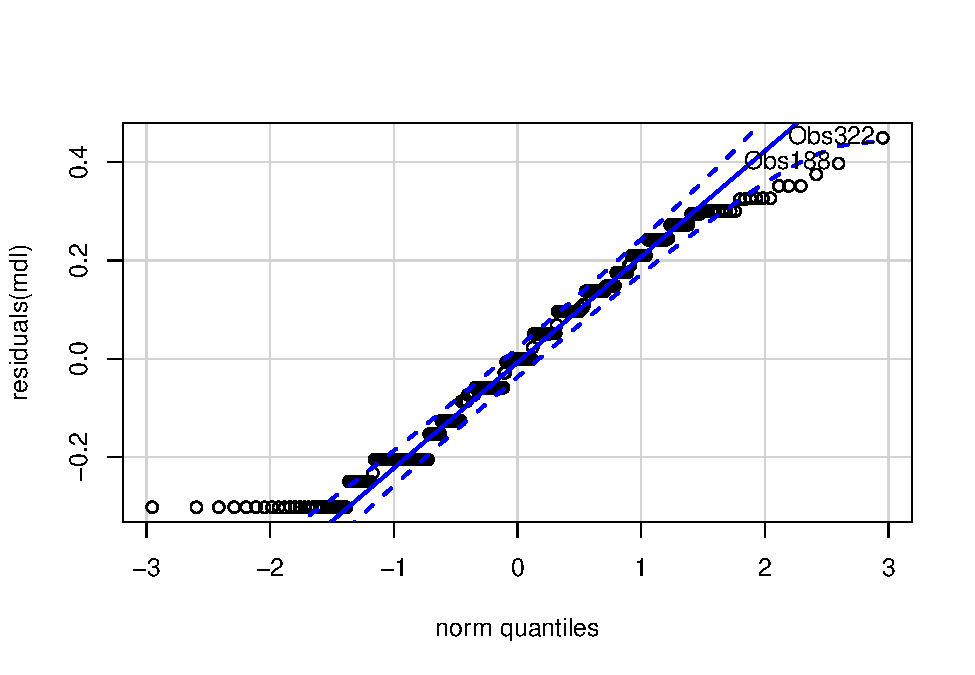
\includegraphics{factorialAnova_files/figure-latex/unnamed-chunk-19-1.pdf}

\begin{verbatim}
## Obs278 Obs239 
##     18     16
\end{verbatim}

\hypertarget{homogeneity-of-variance-assumption}{%
\subsubsection{Homogeneity of variance
assumption}\label{homogeneity-of-variance-assumption}}

\begin{Shaded}
\begin{Highlighting}[]
\KeywordTok{levene_test}\NormalTok{(sdat, }\StringTok{`}\DataTypeTok{desenvolvimento}\StringTok{`} \OperatorTok{~}\StringTok{ `}\DataTypeTok{unidade}\StringTok{`}\NormalTok{)}
\end{Highlighting}
\end{Shaded}

\begin{longtable}[]{@{}rrrll@{}}
\toprule
df1 & df2 & statistic & p & p.signif\tabularnewline
\midrule
\endhead
2 & 316 & 0.211 & 0.8099 & ns\tabularnewline
\bottomrule
\end{longtable}

From the output above, non-significant difference indicates homogeneity
of variance in the different groups (Signif. codes: 0 **** 0.0001 ***
0.001 ** 0.01 * 0.05 ns 1).

\hypertarget{computation-anova}{%
\subsection{Computation ANOVA}\label{computation-anova}}

\begin{Shaded}
\begin{Highlighting}[]
\NormalTok{res.aov <-}\StringTok{ }\KeywordTok{anova_test}\NormalTok{(sdat, }\StringTok{`}\DataTypeTok{desenvolvimento}\StringTok{`} \OperatorTok{~}\StringTok{ `}\DataTypeTok{unidade}\StringTok{`}\NormalTok{, }\DataTypeTok{type =} \DecValTok{2}\NormalTok{, }\DataTypeTok{effect.size =} \StringTok{'ges'}\NormalTok{, }\DataTypeTok{detailed =}\NormalTok{ T)}
\KeywordTok{get_anova_table}\NormalTok{(res.aov)}
\end{Highlighting}
\end{Shaded}

\begin{verbatim}
## Coefficient covariances computed by hccm()
\end{verbatim}

\begin{longtable}[]{@{}lrrrrrllr@{}}
\toprule
Effect & SSn & SSd & DFn & DFd & F & p & p\textless{}.05 &
ges\tabularnewline
\midrule
\endhead
unidade & 0.617 & 219.6 & 2 & 316 & 0.444 & 0.642 & &
0.003\tabularnewline
\bottomrule
\end{longtable}

\hypertarget{post-hoct-tests-pairwise-comparisons}{%
\subsection{Post-hoct Tests (Pairwise
Comparisons)}\label{post-hoct-tests-pairwise-comparisons}}

\begin{itemize}
\tightlist
\item
  Estimated marginal means for \textbf{unidade}
\end{itemize}

\begin{Shaded}
\begin{Highlighting}[]
\NormalTok{(emm[[}\StringTok{"unidade"}\NormalTok{]] <-}\StringTok{ }\KeywordTok{emmeans_test}\NormalTok{(sdat, }\StringTok{`}\DataTypeTok{desenvolvimento}\StringTok{`} \OperatorTok{~}\StringTok{ `}\DataTypeTok{unidade}\StringTok{`}\NormalTok{, }\DataTypeTok{p.adjust.method =} \StringTok{"bonferroni"}\NormalTok{, }\DataTypeTok{detailed =}\NormalTok{ T))}
\end{Highlighting}
\end{Shaded}

\begin{longtable}[]{@{}lllrrrrrrrll@{}}
\toprule
.y. & group1 & group2 & estimate & se & df & conf.low & conf.high &
statistic & p & p.adj & p.adj.signif\tabularnewline
\midrule
\endhead
desenvolvimento & UFAL A.C. Simões & UFAL Arapiraca & 0.1147 & 0.1255 &
316 & -0.1322 & 0.3617 & 0.9141 & 0.3614 & 1 & ns\tabularnewline
desenvolvimento & UFAL A.C. Simões & UFAL CECA & -0.0195 & 0.1784 & 316
& -0.3706 & 0.3315 & -0.1095 & 0.9129 & 1 & ns\tabularnewline
desenvolvimento & UFAL Arapiraca & UFAL CECA & -0.1343 & 0.2045 & 316 &
-0.5366 & 0.2681 & -0.6565 & 0.5120 & 1 & ns\tabularnewline
\bottomrule
\end{longtable}

\hypertarget{descriptive-statistic-and-anova-plots}{%
\subsection{Descriptive Statistic and ANOVA
Plots}\label{descriptive-statistic-and-anova-plots}}

\begin{Shaded}
\begin{Highlighting}[]
\KeywordTok{get_summary_stats}\NormalTok{(}\KeywordTok{group_by}\NormalTok{(sdat, }\StringTok{`}\DataTypeTok{unidade}\StringTok{`}\NormalTok{), }\DataTypeTok{type =}\StringTok{"common"}\NormalTok{)}
\end{Highlighting}
\end{Shaded}

\begin{longtable}[]{@{}llrrrrrrrrr@{}}
\toprule
unidade & variable & n & mean & median & min & max & sd & se & ci &
iqr\tabularnewline
\midrule
\endhead
UFAL A.C. Simões & desenvolvimento & 241 & 2.689 & 2.667 & 1 & 4.333 &
0.827 & 0.053 & 0.105 & 1.333\tabularnewline
UFAL Arapiraca & desenvolvimento & 54 & 2.574 & 2.667 & 1 & 4.333 &
0.815 & 0.111 & 0.222 & 1.000\tabularnewline
UFAL CECA & desenvolvimento & 24 & 2.708 & 2.667 & 1 & 4.667 & 0.939 &
0.192 & 0.397 & 1.083\tabularnewline
\bottomrule
\end{longtable}

\begin{Shaded}
\begin{Highlighting}[]
\KeywordTok{ggPlotAoV}\NormalTok{(sdat, }\StringTok{"unidade"}\NormalTok{, }\StringTok{"desenvolvimento"}\NormalTok{, }\DataTypeTok{aov=}\NormalTok{res.aov, }\DataTypeTok{pwc=}\NormalTok{emm[[}\StringTok{"unidade"}\NormalTok{]], }\DataTypeTok{addParam=}\KeywordTok{c}\NormalTok{(}\StringTok{"jitter"}\NormalTok{))}
\end{Highlighting}
\end{Shaded}

\includegraphics{factorialAnova_files/figure-latex/unnamed-chunk-24-1.pdf}

\hypertarget{references}{%
\subsection{References}\label{references}}

{[}1{]}: Blanca, M. J., Alarcón, R., Arnau, J., Bono, R., \& Bendayan,
R. (2017). Non-normal data: Is ANOVA still a valid option?. Psicothema,
29(4), 552-557.

{[}2{]}: Ghasemi, A., \& Zahediasl, S. (2012). Normality tests for
statistical analysis: a guide for non-statisticians. International
journal of endocrinology and metabolism, 10(2), 486.

{[}3{]}: Miot, H. A. (2017). Assessing normality of data in clinical and
experimental trials. J Vasc Bras, 16(2), 88-91.


\end{document}
